%%%%%%%%%% METHODS %%%%%%%%%%%
\section{Methods}
\label{sec:methods}

% in the vicinty of
% clarify that  flow is highly 3D with wind veering / backing, strong zonal wind higher up stratosphere  favors propagation 

% simulations are simplified for now only considering coriolis effect based on obstacle deflection??

% Maybe include: \\
% - no baroclinic instability simulation -> no baroclinic jet stream \\
% - only barotropic jet

The goal of this thesis is an improved understanding of the processes that lead to observed gravity waves above TDs. A complete three dimensional simulation of the troposphere and stratosphere including all relevant features, more precisely a Rossby wave train and jet stream at the tropopause and a PNJ higher up in the stratosphere to the south, requires challenging initial conditions to obtain suited fields of wind, temperature and pressure (compare section \ref{sec:barocInstability}). Though such a simulation has to be the final step to prove or debunk the described mechanisms, preliminary investigations of simplified simulations likely provide first insights and might significantly help to setup and interpret more complex runs. Therefore, the proposed thesis comprises a selection of simulations with reduced complexity to address parts of the problem step by step.

The fundamental simplification for all preliminary simulations is the focus on dynamics in the stratosphere by introducing the tropopause as the lower boundary of the simulation's domain. It is clear that the tropopause is not an impermeable surface, but observations from radiosondes (\cite{birner_how_2002} and \cite{birner_fine-scale_2006}) and GPS data (\cite{randel_extratropical_2007}) revealed a significantly higher thermal stability of the extratropical tropopause inversion layer compared to model and reanalysis data. This higher stratification further inhibits troposphere-stratosphere exchange at the tropopause and justifies the approach of using the tropopause as the lower boundary for first simulations. The planned simulations and corresponding simplifications are described in the following subsections and summarized in table \ref{tab:simRuns}.

\begin{table*}[]
\caption{EULAG simulation runs}
\begin{tabular}{@{}lll@{}}
\toprule[1pt]
                    & Simulation                                             & Description                                                                                                                                                          \\ \midrule[1pt]
\multirow{19}{*}{2D} & 001: Fundamental flow regimes over orography                & \begin{tabular}[c]{@{}l@{}}- Non-hydrostatic wave regime\\ - Hydrostatic wave regime\\ - Inertia-gravity wave regime \\ \end{tabular}                                                                      \\ \arrayrulecolor{black!30}\cmidrule[1pt]{2-3}
                    & 002: Mtn / TD shape comparison                & \begin{tabular}[c]{@{}l@{}}- Witch of Agnesi\\ - $(1+cos(\phi))$ shape \\ - $(1+cos(\phi))^4$ shape \end{tabular}                                                                      \\ \arrayrulecolor{black!30}\cmidrule[1pt]{2-3}
                    & 003: Transient lower boundary test                              & \begin{tabular}[c]{@{}l@{}}- Mtn rises or moves in $x$-direction \\ - No background wind  \\ - Test smooth start up / end of motion \end{tabular}        \\ \cmidrule[1pt]{2-3}
                    & 004: Transient TD like Prusa et al. (2003)               & \begin{tabular}[c]{@{}l@{}}- Oscillating TD in zonal direction \\ - Constant stratospheric background wind \\ - Constant stratospheric stability \end{tabular}         \\ \cmidrule[1pt]{2-3}
                    & 005: Propagating TD with vertical shear  & \begin{tabular}[c]{@{}l@{}} - PNJ at $\approx 40$km  \\ - TD moves with phase velocity of Rossby wave \\ - Design idealized wind profile \\ - Use wind profile from ECMWF \\ - \textbf{Sensitivity analysis} wrt. shape of depression \\ ($h_0$, $a$ and asymmetry)    \end{tabular}      \\ \cmidrule[1pt]{2-3}
                    & 006: Propagating TD with meridional wind & \begin{tabular}[c]{@{}l@{}} - Run 2D005 with Coriolis force \end{tabular}        \\ \arrayrulecolor{black}\cmidrule[1pt]{1-3}
\multirow{11}{*}{3D}                 & 007: Propagating TD with vertical shear                & \begin{tabular}[c]{@{}l@{}} - Run 2D005/006 in 3D  \\ - TD oriented N-S \\ - Compare elongated and local depression \\ (elliptic shape) \end{tabular}   \\ \arrayrulecolor{black!30}\cmidrule[1pt]{2-3}
                    & 008: Tilted TD with vertical shear                     & \begin{tabular}[c]{@{}l@{}} - Run 3D007 with tilted TD (oriented NW-SE)  \end{tabular}       \\ \cmidrule[1pt]{2-3}
                    & 009: Barocl. (or barotropic) PNJ above TD  &  \begin{tabular}[c]{@{}l@{}} - Include horizontal shear \\ - 2D Gaussian distribution (for barocl. jet) \\ - $\theta_{env}$ from thermal wind relation (for barocl. jet) \\ - PNJ directly above tropopause depression  \end{tabular}    \\ \cmidrule[1pt]{2-3}
                    & 010: Barocl. (or barotropic) PNJ shifted south   & \begin{tabular}[c]{@{}l@{}} - Simulation 3D009 with PNJ shifted south \end{tabular}      \\ \cmidrule[1pt](l){2-3} 
                    & 011: Full simulation including troposphere                  & \begin{tabular}[c]{@{}l@{}}- Initialisation based on Bush et al. (1994)\\ - Extension of barocl. instability with PNJ\end{tabular}     \\
                    \arrayrulecolor{black}\bottomrule[1pt]
\end{tabular}
\label{tab:simRuns}
\end{table*}

\subsection{Model setup and verification}
\label{sec:modelVerification}

% 8). In effect, the characteristic Froude number Fr = N hm /U = 0.1 < 1. Therefore, according to [36], we can expect that the steady nonlinear solution of the numerical simulations is close to the linear one.

Simulations 2D001-2D004 of table \ref{tab:simRuns} ensure that the model is setup correctly and provides physically reasonable outputs. In that sense, it is the goal to reproduce some fundamental analytic results based on linear theory with nonlinear EULAG simulations. \textcite{queney_problem_1948} was the first to summarize different flow regimes over mountains based on the method of small adiabatic perturbations. His results can be compared to simulations from a visual perspective by looking at the perturbations and fluxes in the atmosphere and from a mathematical one by comparing the wave drag
%
\begin{equation}
    \mathcal{F} = \int_{}^{} p^{'} \frac{\partial h}{\partial x} dx
    \label{equ:waveDrag}
\end{equation}
%
to its analytic solution in a linear framework (\cite{gill_atmosphere-ocean_1982}). Assuming an impermeable tropopause at the lower boundary of the simulations results in a TD that acts like a flipped mountain (valley) on the stratosphere, so a comparison of our model to Queney's solutions for different mountain wave regimes (non-hydrostatic, hydrostatic, inertia-gravity) provides a reasonable baseline and validation of the model for the planned simulations.

Depending on the application or numerical problem at hand, the function, that describes the surface boundary (mountain shape) can have useful or disturbing properties. The Witch of Agnesi

\begin{equation}
    h_{Agnesi}(x) = \frac{h_0}{(\frac{x}{a})^2+1}
    \label{equ:witchOfAgnesi}
\end{equation}

used by \textcite{queney_problem_1948} is a convenient equation of the terrain height for analytical analysis, but it is non-zero for the whole domain of discrete simulations. In the case of a transient lower boundary this effect leads to inconsistent boundary conditions at the horizontal borders, making this a less appropriate shape for a propagating TD. A suitable alternative is a $1+cos(\pi \phi)$ function. It drops to 0 for $|\phi| = 1$. With 
%
\begin{equation}
    h_{cos}(\phi) = \frac{h_0}{16} (1+cos(\pi \phi))^4
    \label{equ:cosMtn}
\end{equation}
%
and $ \phi = \frac{x}{4a}$ \textcite{epifanio_three-dimensional_2001} used a variation of this function, which is more comparable to the Witch of Agnesi (\ref{equ:witchOfAgnesi}). Setting $h_{cos}(\phi)=0$ for all grid points $|x| > 4a$ results in a continuous and differential lower boundary that does not interfere with horizontal boundary conditions as long as the mountain or depression is not too close to the edges. Furthermore, all contributions to the surface pressure drag are confined to a small neighbourhood around the mountain peak. \textcite{metz_are_2021} state that the wave drag is a factor 1.3 higher compared to the Witch of Agnesi, but further comparisons of the terrain functions and their impact on the overlying flow are carried out (simulation 2D002).

In simulations 2D003 it is the goal to observe the propagation of waves for a rising and for a moving lower boundary in an atmosphere at rest. With no background wind and a constant static stability the simulation is expected to mimic the perturbations in a water tank, when for example pulling an obstacle at the bottom through the quiescent fluid. Furthermore, in this way the linearized governing equations simplify even further and it might be possible to identify patterns in the waves' group ($c_g$) and phase velocities, which are characteristic for the scenario without a background flow. For example the parallel orientation of $c_g$ to the wave's phase lines and the corresponding direction of the energy propagation (\cite{lin_mesoscale_2007}).

For a last physical validation it is appropriate to start two-dimensional simulations of a transient TD by reproducing the simulations of a zonally oscillating TD conducted by \textcite{prusa_all-scale_2003} (simulation 2D004 in table \ref{tab:simRuns}). They showed that inertia-gravity waves are constantly observable above a TD ($h_0$=\SI{500}{\meter}, $a$=\SI{200}{\kilo\meter}) for a constant stratospheric background wind of \SI{10}{\meter\per\second}, a constant buoyancy frequency $N$ of \SI{0.02}{\second^{-1}} and an isothermal stratosphere. However, the waves above the TD are expected to change continuously, because the relative speed of the depression with respect to the constant background wind changes, too. In particular, the varying tilt of the phase lines should be observable. 

\subsection{2D simulations of a propagating tropopause depression}
\label{sec:2D}

The next step in the two-dimensional space is the introduction of a realistic stratospheric wind profile (simulation 2D005 in table \ref{tab:simRuns}). Two approaches are possible. The first one incorporates the design of idealized profiles with increasing complexity. At first, a PNJ could be represented by a Gaussian distribution peaking at a level between 40-\SI{50}{\kilo\meter}. In a next step, it could be of interest to add a second jet at the tropopause level resulting in a negative wind shear in the lower stratosphere before the wind increases again higher up. For this purpose, a higher order function approximation might be more suited than a superposition of two Gaussian distributions to avoid sharp changes in the vertical shear. Environmental profiles of $\theta$, $T$ or $p$ still refer to a constant stability and an isothermal atmosphere. The second approach relies on realistic ECMWF wind profiles, which are already available from the observational analysis of RF25 of the DEEPWAVE campaign (\cite{dornbrack_stratospheric_2021}). These profiles represent meridional means of a relevant 5$\degree$ wide latitude band and naturally include complex shear scenarios due to the PNJ and the tropopause jet stream. 

For these simulations (2D005) it is planned to reduce the movement of the TD to a constant propagation from left to right through the simulation domain. In this way, the effect of vertical wind profiles on the excitation and propagation of waves above a transient TD is not disturbed by an unrealistic movement of the depression. At the upper and lateral boundaries, the vertical and horizontal radiation of wave energy is treated by relaxation terms as further described in section \ref{sec:EULAG}. The parameters of these damping layers are tuned to reduce boundary effects like wave reflection to a minimum.

At this point, it is also planned to conduct a sensitivity analysis with respect to the depression's shape. Effects of its depth, width and possibly asymmetry shall be investigated. The settings used by \textcite{prusa_all-scale_2003} serve as a good starting point, but observations (\cite{bush_tropopause_1994} and \cite{keyser_review_1986}) and reanalysis data (\cite{dornbrack_stratospheric_2021} and \cite{skerlak_tropopause_2015}) suggest quite a range of realistic parameters. This sensitivity analysis can provide first hints on expected wave regimes and help to identify optimal settings for further simulations.

Simulation 2D006 is closely related to 2D005 with the difference of activating the Coriolis force and allowing meridional winds. All other settings will be left unchanged with respect to a reference simulation of 2D005 to directly observe differences in the wave excitation and propagation.  

% Cyclic boundary conditions?? interaction with boundaries again! 

% cite RF25 paper for profiles

% max. wind speed between 40-80 m/s (\cite{bush_tropopause_1994}) \\

% phase velocity 8.7 m/s in RF25 paper??? actual speed of depression varies
% (four times higher stability compared to tropospheric  
% basic state equaled environmental state

% include meridional wind speed. Jet stream to the NE of fold (orientation NW-SE) 
% northward v component before depression, southward v component after

%%%% 3D %%%%%
\subsection{3D simulations of a propagating TD}
\label{sec:3D}

The first three-dimensional simulations are extending simulations 2D005 and 2D006 into the meridional dimension with a focus on the shape of the TD. As described in section \ref{sec:propagation}, two mechanisms are able to describe the meridional propagation of GWs into the PNJ at 60$\degree$S. A non-parallel wave vector with respect to the background zonal wind and horizontal wind shear. Neglecting horizontal wind shear for simulations 3D007 and 3D008 allows the isolated investigation of a meridional propagation due to the orientation of the wave vector. In that manner, it is the goal to compare differences in wave propagation between an elongated N-S oriented depression, a N-S oriented, local depression (elliptic shape) and a tilted (NW-SE), local depression (simulation 3D008). The background wind for simulations 3D007 and 3D008 will be the same as in 2D005 and constant in meridional direction. Meridional winds only appear based on the Coriolis force, the environmental $V$ component is zero. 

Simulations 3D009 and 3D010 are addressing the second mechanism for horizontal wave propagation, the horizontal wind shear. In addition to the vertical wind shear, it is now the goal to design a baroclinic jet system with vertical and horizontal shear. Thus, the environmental $U$ component varies in horizontal and vertical direction, while the background meridional wind $V$ is still zero. Most likely, a reasonable wind field can be obtained by a two-dimensional Gaussian distribution. Simulation 3D009 is then planned to have the PNJ directly above the tropopause depression to provide a reference simulation for simulation 3D010 that finally has a baroclinic PNJ south of the tropopause depression. 

When introducing a baroclinic jet with horizontal and vertical wind shear as a background (environmental) wind field, its influence on the environmental state of the atmosphere has to be considered. The potential temperature distribution now has to balance the gradients in the wind field on the basis of the thermal wind relation
%
\begin{equation}
    \frac{\partial U}{\partial z} = -\frac{g}{\theta_0 f} \frac{\partial \theta}{\partial y}
    \label{equ:thermalWind}
\end{equation}
%
with $g$ and $f$ being the gravitational acceleration and Coriolis parameter and $\theta_0$ a constant basic state reference temperature. In the case of an isothermal stratosphere the pressure and density fields are fully defined, but further options might be investigated.

An additional simplification for 3D009 and 3D010 could be a barotropic jet with horizontal shear only instead of a baroclinic PNJ. Vertical wind shear would be zero, but the PNJ can still be positioned above the TD (3D009) and further to the south (3D010) to observe differences in the wave propagation with respect to the horizontal gradient in the wind.
% begin{equation}
%     u(\phi)=u_0 sin^3(\phi) cos(\phi)
% \end{equation}

%%%% Baroclinic instability %%%%
\subsection{Full simulation including troposphere}
\label{sec:barocInstability}

Though this final simulation (3D011) of the troposphere and stratosphere is most likely not covered within the proposed thesis, it is still mentioned at this point for the sake of completeness. It comprises the simulation of a baroclinic instability at the tropopause, as already carried out by \textcite{bush_tropopause_1994}, with the crucial difference of a PNJ in the upper stratosphere to the south. Though \textcite{bush_tropopause_1994} cover all relevant equations to define a balanced field that allows the initialisation of a baroclinic jet simulation, it is far from trivial to additionally consider a PNJ. 

 

\chapter{Meridional propagation of GWs excited by tropopause depressions}
\label{sec:results3D}

Eventually eight full 3D simulations were conducted to investigate the effect of a tilted TD and horizontal wind shear on the meridional propagation of GWs.
Three simulations without horizontal shear an


Add another simulation with a stronger PNJ and stronger horizontal shear to observe 
\section{Effects of TD orientation in atmosphere}
% no meridional shear


\section{Variations of the TD's zonal width and its effect on the meridional propagation of GWs}

extrinsic frequency is conserved along the ray. Is 0 for stationary mountain waves.

intrinsic frequency = 




\section{The impact of rotating the TD with respect to the zonal}
% no meridional shear

- Wavelet analysis described earlier

- 

\begin{figure*}[tbp]
    \centering
    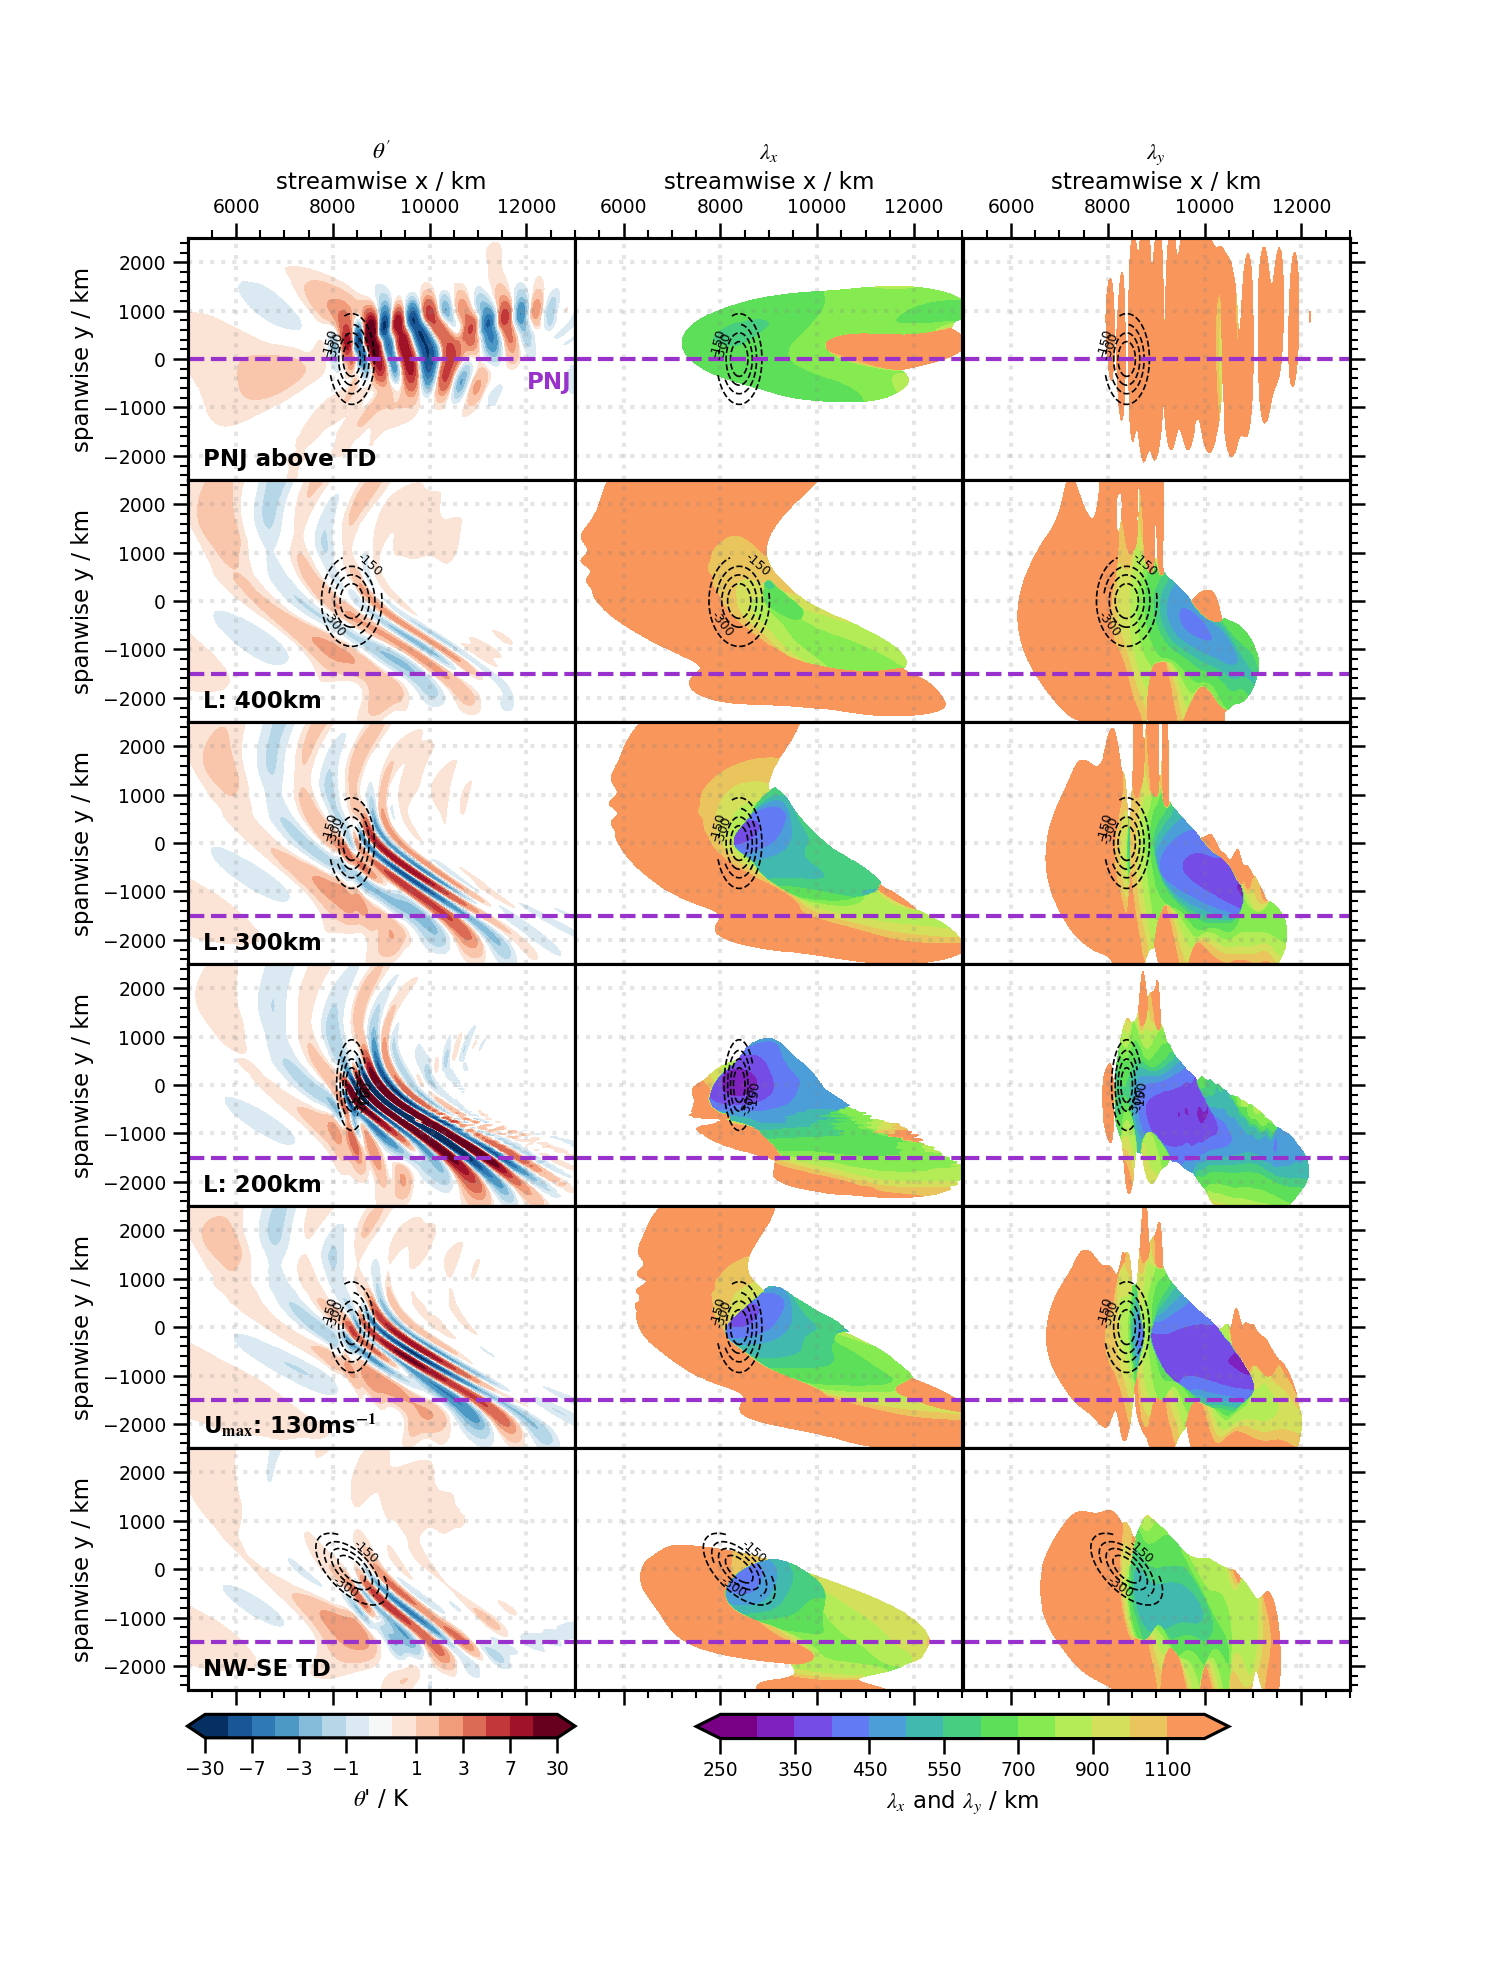
\includegraphics[width=0.99\textwidth]{figures_3D/waveletAna_dudy.png}
    \caption{Horizontal cross sections at 40km above the tropopause for five simulations with horizontal and meridional shear in a barotropic environment. Shown are $\theta$', $\lambda_x$ and $\lambda_y$ at 72h into the simulation. Dominant zonal and meridional wavelengths for each grid point are determined from wavelet analysis.}
    % \label{fig:waveletAna_dudy}
\end{figure*}


\section{Momentum fluxes from a simulation-based and observational perspective}

MF$_x$ MF$_y$ can be calculated directly from wind perturbations ($u'$, $v'$,$w'$) provided by the numerical simulation with the EULAG model. However, most satellite or ground-based observations measure temperature perturbations without further information on the corresponding wind (e.g. \cite{hindley_gravity_2019}, \cite{kaifler_compact_2021}, \cite{wu_satellite_1996}). For 2D Lidar observations these measurements usually aren't sufficient to derive horizontal momentum fluxes without additional information or assumptions for horizontal wavelengths. In the case of three dimensional datasets, as analysed by \textcite{hindley_18year_2020} (satellite observations), the determination of momentum fluxes is possible under the midfrequency approximation. This analysis follows \textcite{ern...} and combines the calculation of the potential energy (equation PE) with a three dimensional spectral analysis to obtain corresponding wavenumbers. Zonal and meridional momentum fluxes are 

\begin{equation}
    (\mathrm{MF}_x, \mathrm{MF}_y) = \frac{\rho}{2} (\frac{g}{N})^2 (\frac{T'}{\bar{T}})^2 (\frac{k}{m},\frac{l}{m})
\end{equation}

% with $\rho$ being the density, $g$ the gravitational acceleration, N the Brunt‐Väisälä frequency, $T'$ and $\bar{T}$ temperature perturbations and background temperature respectively and $k,l,m$ are zonal, meridional and vertical wavenumbers (\cite{ern}). This relation is valid for hydrostatic and nonrotational GWs with an intrinsic frequency in the range $f \ll \hat{\omega} \ll N$, where $f$ is the inertial frequency (e.g., Fritts & Alexander, 2003).

Maybe it makes sense that MFx via wavelet analysis is smaller, because it collapses contribution to a single frequency

\begin{figure*}[tbp]
    \centering
    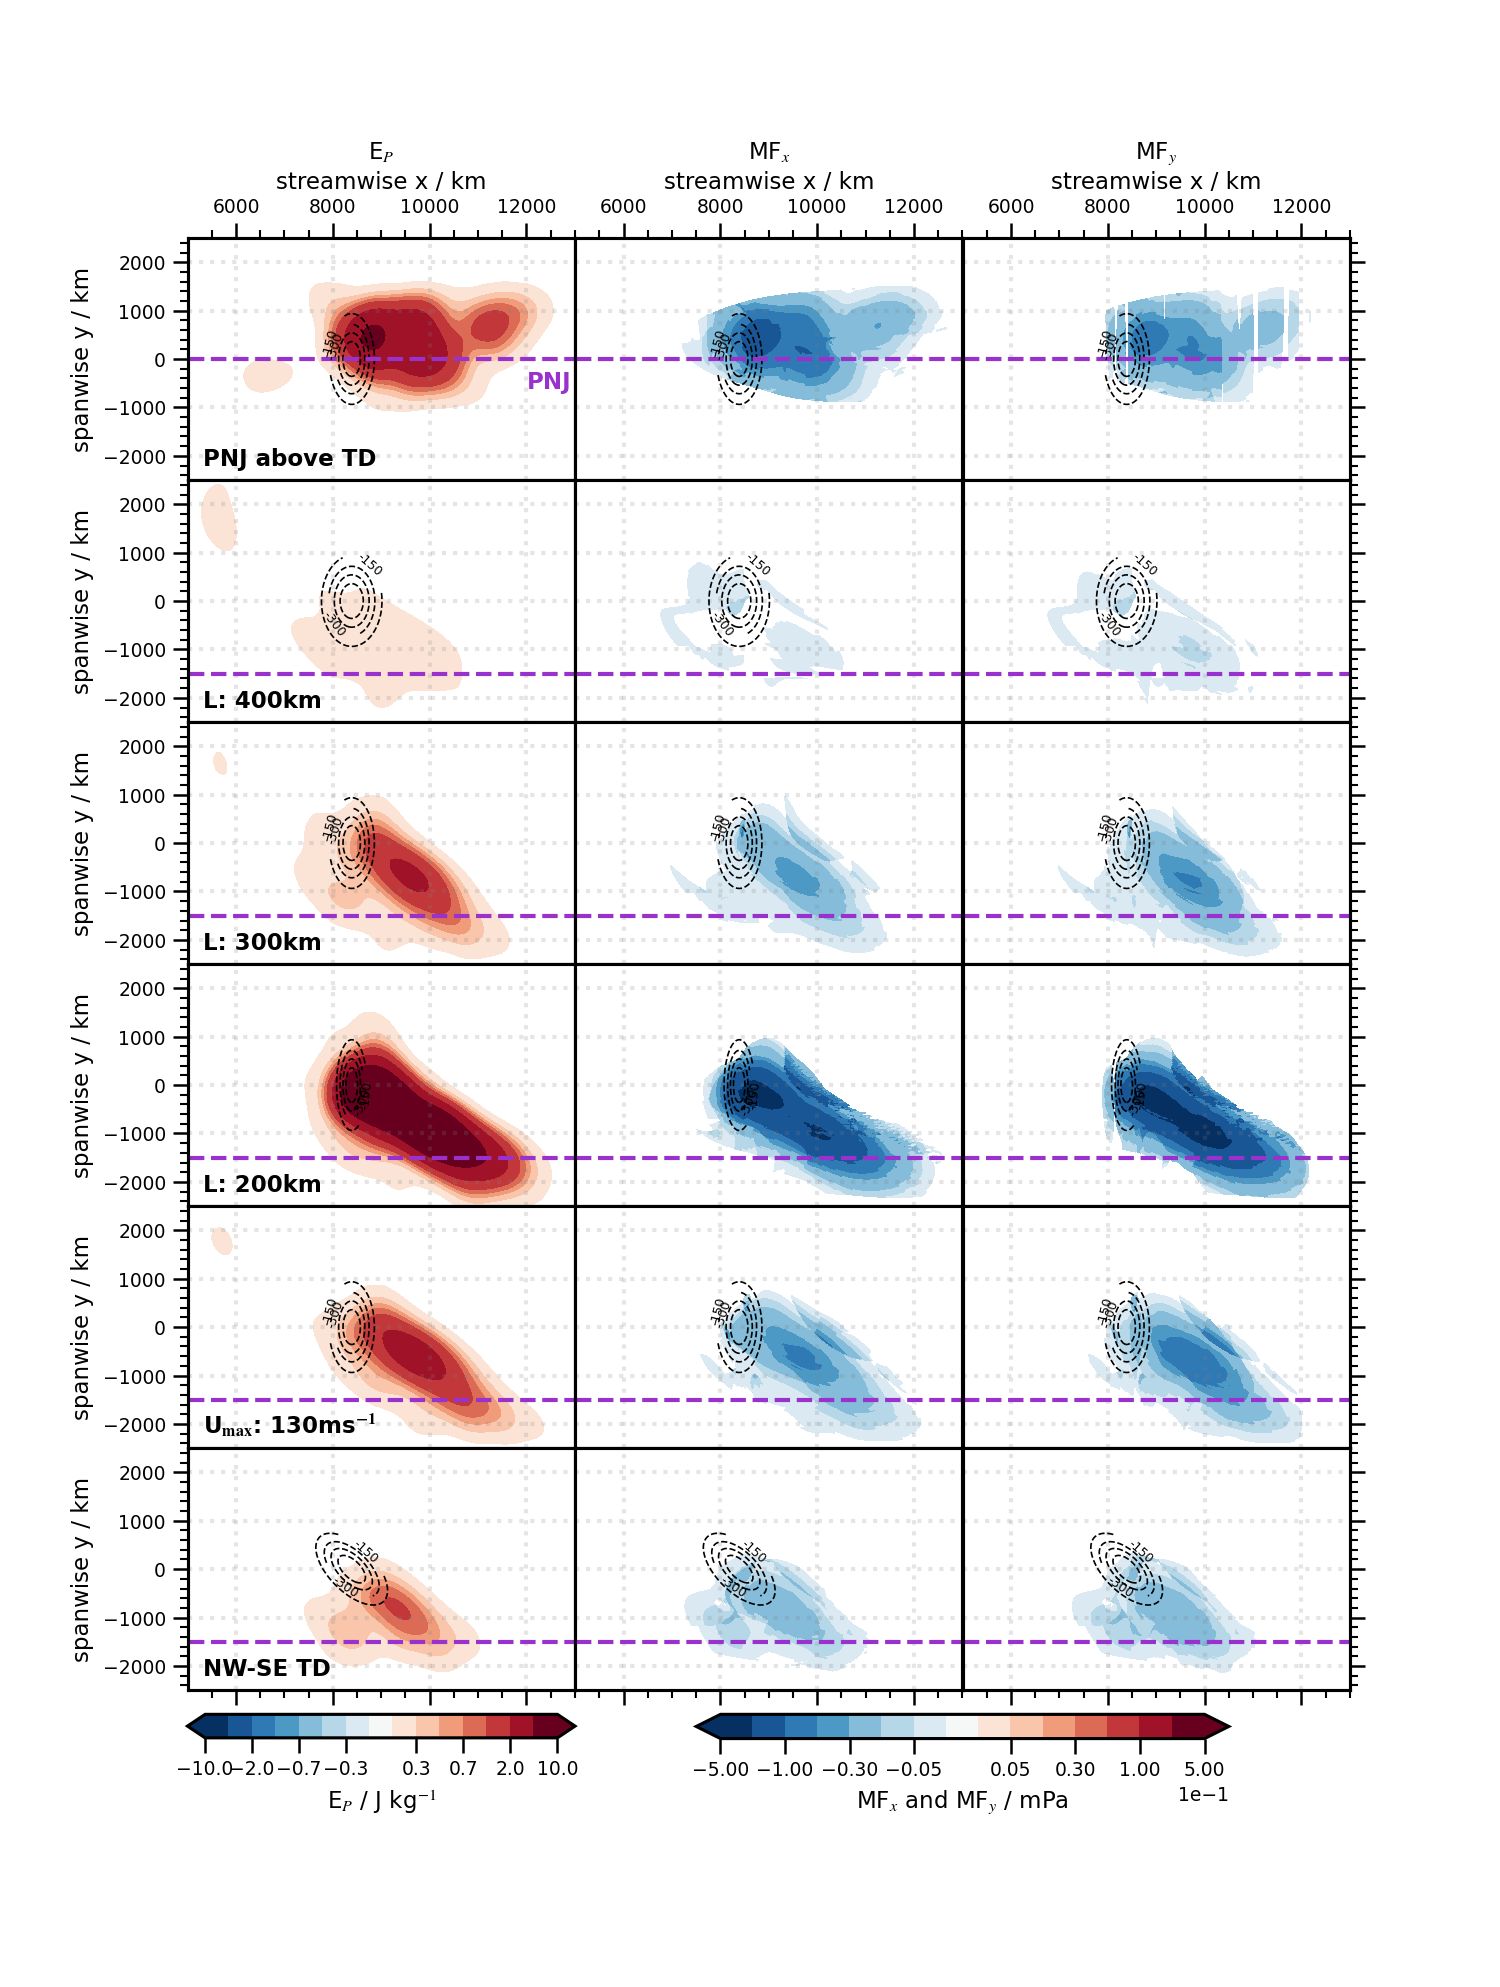
\includegraphics[width=0.99\textwidth]{figures_3D/waveletAna_fluxes_obs.png}
    \caption{Horizontal cross sections at 40km above the tropopause for five simulations with horizontal and meridional shear in a barotropic environment. Shown are $\theta$', $\lambda_x$ and $\lambda_y$ at 72h into the simulation. Dominant zonal and meridional wavelengths for each grid point are determined from wavelet analysis.}
    % \label{fig:waveletAna_dudy}
\end{figure*}

\begin{figure*}[tbp]
    \centering
    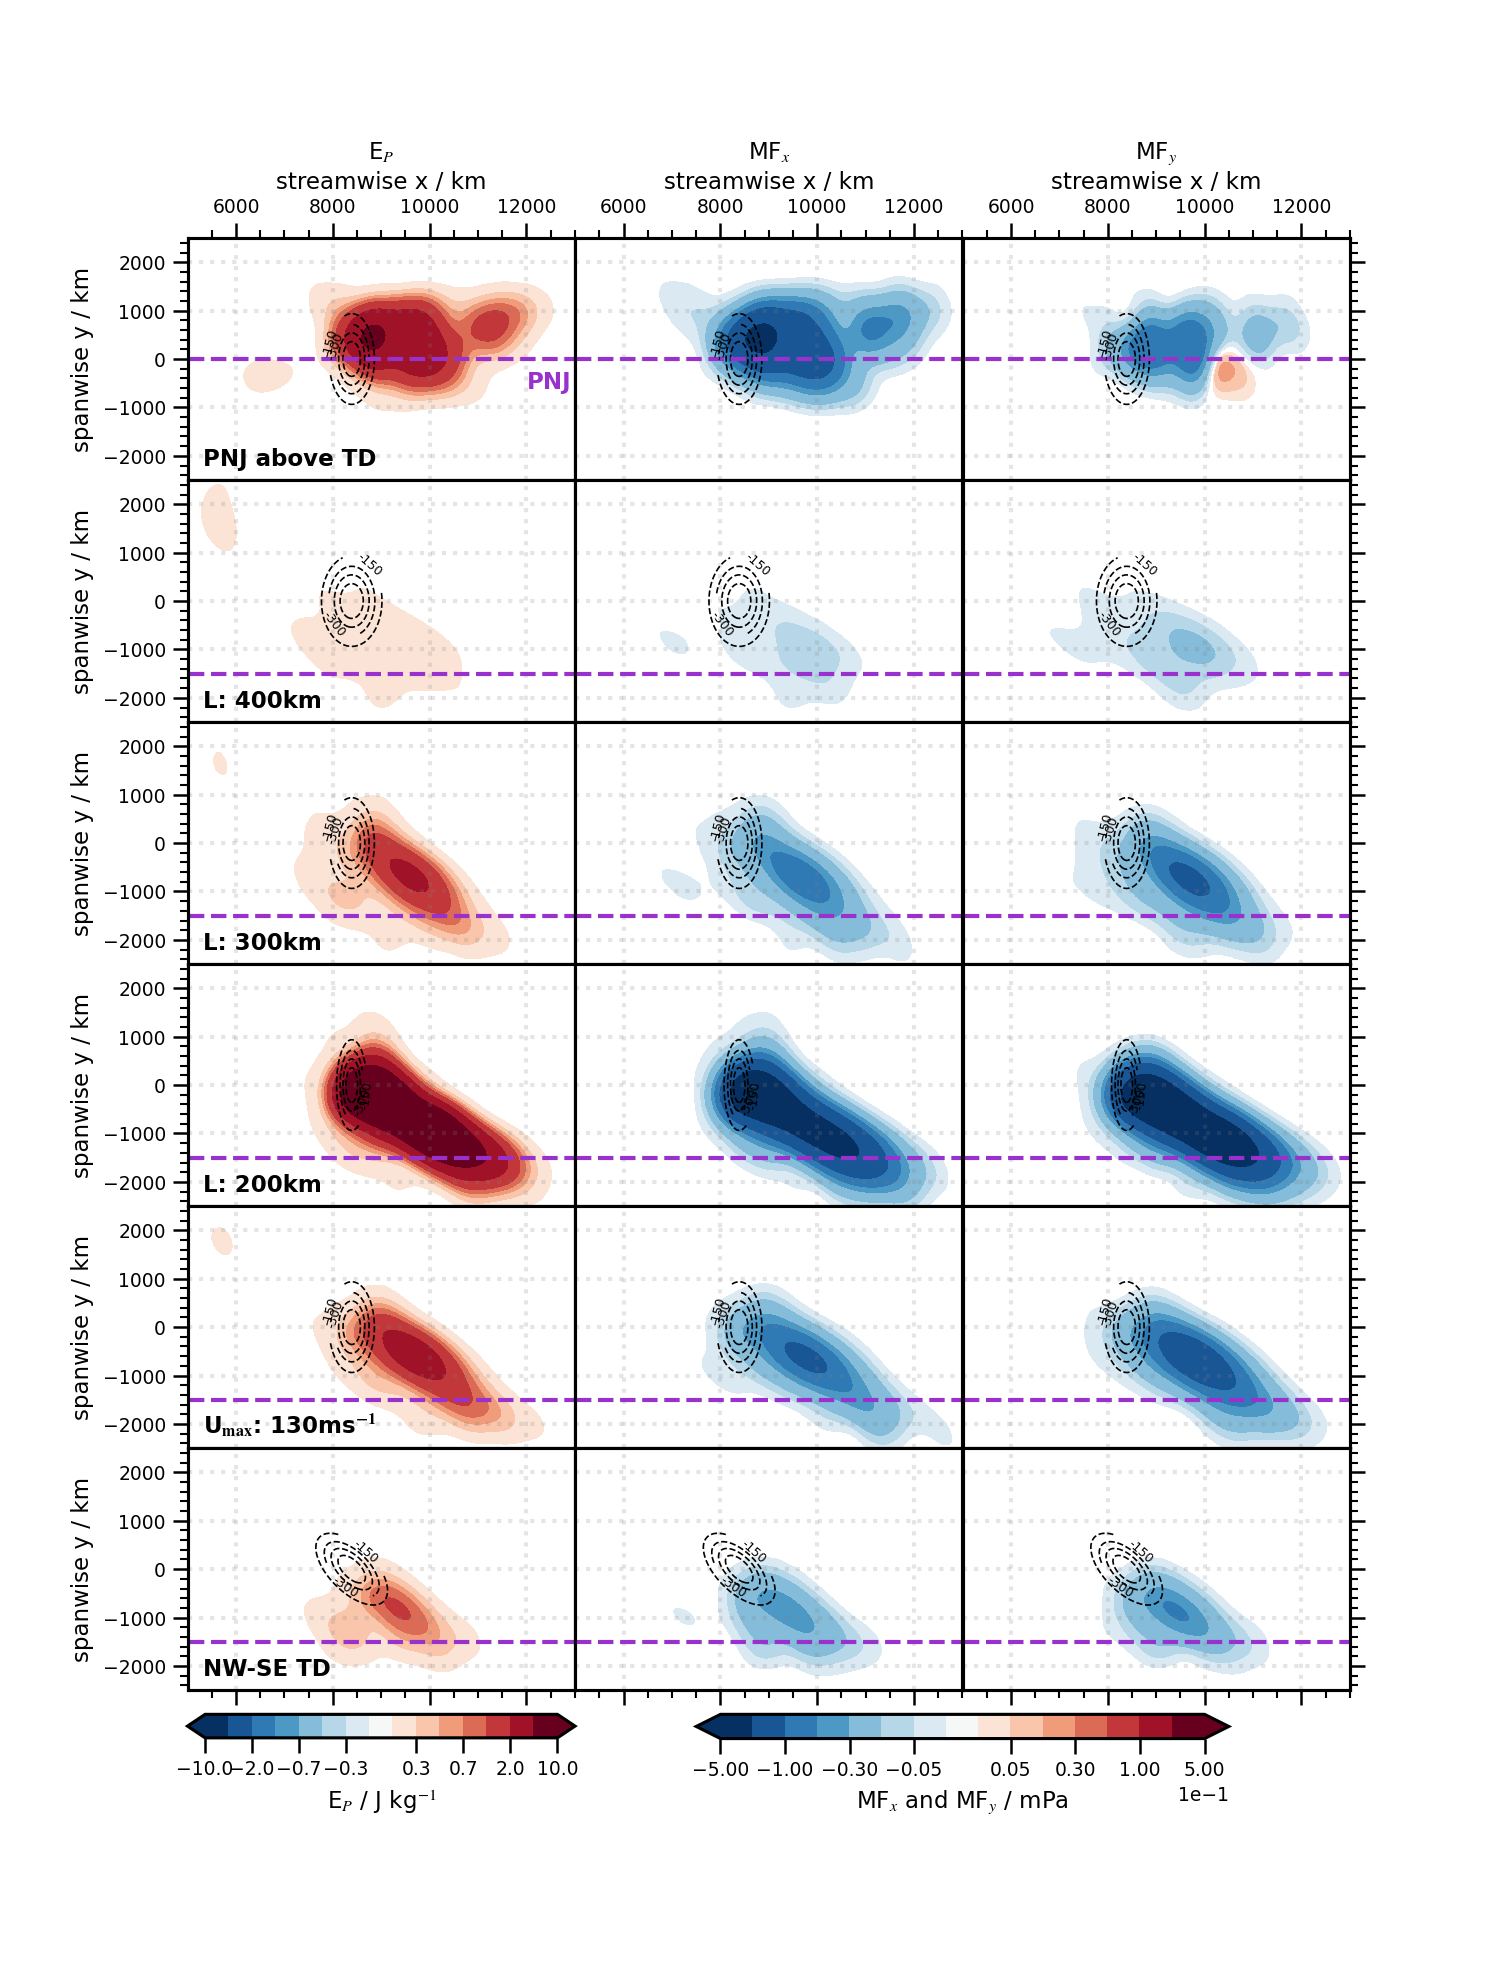
\includegraphics[width=0.99\textwidth]{figures_3D/waveletAna_fluxes_sim.png}
    \caption{Horizontal cross sections at 40km above the tropopause for five simulations with horizontal and meridional shear in a barotropic environment. Shown are $\theta$', $\lambda_x$ and $\lambda_y$ at 72h into the simulation. Dominant zonal and meridional wavelengths for each grid point are determined from wavelet analysis.}
    % \label{fig:waveletAna_dudy}
\end{figure*}


%%%%%%%%%%%%%%%% COMMENT (PRELIMINARY RESULTS) %%%%%%%%%%%%%%%%%%%%%

\begin{comment}



\subsection{Linear regimes}
\label{sec:linearRegimes}


take description of waves from gill and queney!! 

hydrostatic case waves above mountain with wavelength....

non-hydrostatic lee waves 




\begin{table*}[h]
\centering
\caption{Parameters for the numerical simulations: mountain width L, spatial increments $\Delta$x and $\Delta$z in the horizontal and vertical directions, time step $\Delta$t, thickness $\delta$x$_{ab}$ and time scale $\tau_x$ of the horizontal and altitude z$_{ab}$ and time scale $\tau_z$ of the vertical absorbers.}

\begin{tabular}{@{}lcccccccc@{}}
\toprule
Wave regime & L/km & $\Delta$x/m & $\Delta$z/m & $\Delta$t/s & $\delta$x$_{ab}$/km & $\tau_x$/s  & z$_ab$/km & $\tau_z$/s \\ \midrule[1pt]

Non-hydrostatic & 1 & 100 & 100 & 5 & 24 & 1800 & 38 & 900 \\
Hydrostatic & 10 & 1000 & 100 & 5 & 240 & 300 & 38 & 900 \\
Inertia-Gravity & 100 & 5000 & 100 & 60 & 1200 & 300 & 38 & 3600 \\

\bottomrule
\end{tabular}
\label{tab:linearRegimes}
\end{table*}

\begin{itemize}
    \item h$_m$ = 100 m
    \item U = 10 m s$^{-1}$
    \item N = 0.01 $s^{-1}$ (Brunt–Väisälä frequency)
    \item f = 1.03$\cdot 10^{-4}$ = 1.457$\cdot 10^{-4}$ $\cdot \sin{45°} \approx$ 0.01 N (compare with figure from Gill)
\end{itemize}


\subsection{Comparison of surface shapes} %Q Witch of Agnesi vs. Cos^4

The background flow, or more precisely the wind speed u and stability N (Brunt-Vaisalla frequency) of the atmosphere, define the vertical wavelength of hydrostatic waves that develop for flows over a mountain ridge (Equation \ref{equ:lambdaz}).

\begin{equation}
    N^2 = g \cdot st
    \label{equ:N}
\end{equation}

\begin{equation}
    \lambda_z = \frac{2\pi U}{N}
    \label{equ:lambdaz}
\end{equation}


\subsection{Perturbations in a quiescent fluid}

% Simplifications:

hydrostatic assumptions
geostrophic assumption

only valid as long as perturbations are small (linearization)

Bousinessq approximation

taylor Goldstein equation

\cite{NappoOrLin2007}

(constant buoyancy frequency N of 0.01 $\frac{1}{\textrm{s}}$)

Group velocity parallel to constant phase lines... -> show energy propagation and phase lines

phase velocity perpendicular to group vel

wave number vector points in direction of phase velocity

energy upward and right, phase downward and right


\begin{equation}
    c_x = \frac{\omega}{k} = u_0 \pm \frac{N}{\sqrt{k^2+m^2}}
    \label{equ:cx}
\end{equation}

\begin{equation}
    c_z = \frac{\omega}{z} = u_0 \frac{k}{m} \pm \frac{k N}{m\sqrt{k^2+m^2}}
    \label{equ:cz}
\end{equation}

\begin{equation}
    c_{gx} = u_0 \pm \frac{N m^2}{(k^2+m^2)^{\frac{3}{2}}}
    \label{equ:cgx}
\end{equation}

\begin{equation}
    c_{gz} = u_0 \pm \frac{N k m}{(k^2+m^2)^{\frac{3}{2}}}
    \label{equ:cgz}
\end{equation}


% \include{timeSchedule}





\begin{enumerate}[label=\Alph*]
    \item Verification
    \begin{enumerate}[label=\roman*] % (\arabic*)
        \item Elementary flow regimes
        \item 2D moving lower topography
    \end{enumerate}
    \item Tropopause represents lower boundary of simulation
    \begin{enumerate}[label=\roman*] % (\arabic*)
        \item 2D simulation of moving tropopause depression
        \item 3D simulation of moving tropopause depression without polar night jet
        \item 3D simulation of moving tropopause depression with polar night jet
    \end{enumerate}
    \item Full simulation including troposphere part of simulation
\end{enumerate}


\end{comment}